\documentclass[journal,12pt,twocolumn]{IEEEtran}

\usepackage{enumitem}
\usepackage{amsmath}
\usepackage{amssymb}
\usepackage{graphicx}
\title{Assignment 2 \\ \Large AI1110: Probability and Random Variables \\ \large Indian Institute of Technology Hyderabad}
\author{Pranav B \\ \normalsize AI21BTECH11023 \\ \vspace*{20pt} \normalsize  10 April 2022 \\ \vspace*{20pt} \Large ICSE 2019 Grade 12}
\begin{document}
	% The title
	\maketitle
	
	% The question
	\textbf{Question 7)} 
	A 13 m long ladder is leaning against a wall, touching the wall at a certain height from the ground level.The bottom of the ladder is pulled away from the wall,along the ground at the rate of 2 $m/s$. How fast is the height of the ladder decreasing when the foot of the ladder is 5 m away from the wall?\\
	% The solution
	\textbf{Solution.}
	The various parameters involved in this question are listed in Table \begin{table}[h]
\caption{Variables used}
\begin{tabular}{|c|c|c|}
\hline
Parameter & Variable & value\\
\hline
length of the rod & $s$ & 13 m\\
\hline
height from ground level to tip of rod & $h$ & ???\\
\hline
distance from the wall to foot of rod & $x$ &???\\
\hline
\end{tabular}
\end{table}
\\
\begin{figure}[h]
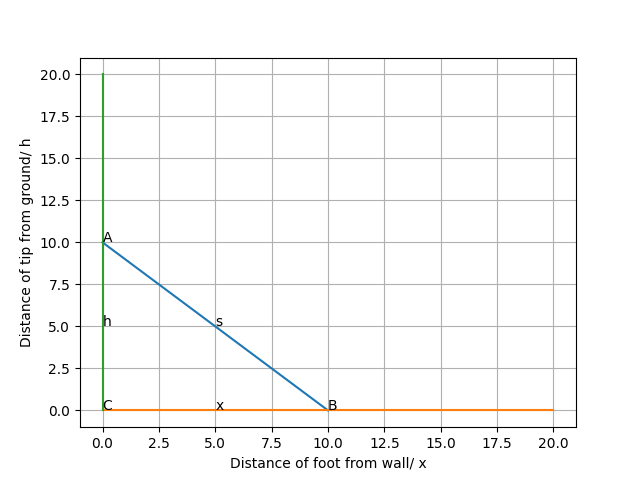
\includegraphics[width=0.3\textwidth]{Pic2}
\caption{Figure depicting the ladder:AB=$s$,BC=$x$,AC=$h$}
\label{fig:my_label}
\end{figure}
\\
\underline{\textbf{Baudhāyana Sulba Sūtra:}}
States that, if given a rectangle of side lengths $a$,$b$ and diagonal length $c$ the sum of the area of squares made by the side lengths of rectangle equals the area of square made by the length of the diagonal of the rectangle.\\
\begin{align}
\implies a^2+b^2=c^2
\end{align}
\\
In Figure-1, we can draw lines parallel to the ground and wall passing through the tip and foot of ladder respectively to get an imaginary rectangle with side lengths $h$,$x$ and diagonal length $s$\\
From Baudhāyana Sulba Sūtra,we get :
\begin{align}
h^2+x^2=s^2
\end{align}
in this equation $s$ is always constant,
 $\because$ length of rod never changes\\
 Now differentiating the equation on both sides with respect to time gives us\\
 \begin{align}
 \frac{d(h^2+x^2)}{dt}=\frac{d(s^2)}{dt}\\
  \implies 2h\frac{dh}{dt}+2x\frac{dx}{dt}=0\\
 \implies h\frac{dh}{dt}=-x\frac{dx}{dt}
 \end{align}
 Given, at some time t=t$_0$,
  $\frac{dx}{dt}$=2 $m/s$ and $x= 5 m$\\
  From Baudhāyana Sulba Sūtra , at time t$_0$
  \begin{align}
  5^2+h^2=13^2
  \end{align}
  $\therefore h= 12 m$\\
  Now from equation (4) substituting $h,x,\frac{dx}{dt}$,we get\\
  \begin{align}
   \frac{dh}{dt}=-\frac{5}{6} m/s
\end{align}  
The negative sign indicates that h is decreasing,
$\therefore$ the height of the ladder is decreasing at a rate of $\frac{5}{6} m/s$
\end{document}